\documentclass[a4paper]{article}
\linespread{1.6}
\usepackage{enumerate}
\usepackage{geometry}
\usepackage{setspace}
\usepackage{amsmath}
\usepackage{amssymb}
\usepackage{algorithm}
\usepackage{algorithmicx}
\usepackage{algpseudocode}
\usepackage[pdftex]{graphicx}
\usepackage{float}
\usepackage{subfigure}
\usepackage{listings}

\usepackage{algpseudocode}
\geometry{left=1.2cm,right=1.2cm,top=2.5cm,bottom=2.5cm}

\floatname{algorithm}{Algorithm}
\renewcommand{\algorithmicrequire}{\textbf{Input:}}
\renewcommand{\algorithmicensure}{\textbf{Output:}}

\begin{document}
\begin{spacing}{2.0}
\begin{flushleft}\begin{huge}EEE6512 Image Processing and Computer Vision   Homework 3\end{huge}\end{flushleft}
\begin{flushright}\begin{Large} Hudanyun Sheng \end{Large}\end{flushright}

\section*{\huge\textbf{ Part \uppercase\expandafter{\romannumeral1} Textbook Questions}  }
	\normalsize

	\textbf{3-16} If histogram equalization is applied twice to an image, that is, if it is applied to the result of histogram equalization, will the second application change the image or not? Explain why or why not.\\

	If histogram equalization is applied to the result of histogram equalization, the second application will not change the image. Compared between an image after histogram equalization 		and before histogram equalization, we know that: (1) the portion for pixels having nonzero values remain the same; (2) the relative intensity of two pixels would remain the same,			 i.e. the one having larger intensity value will still having the comparatively larger intensity. So after one application of histogram equalization, the histogram of the image has already 		been equalized, so the second application change the image.\\
	
	\noindent
	\textbf{3-17} Compute the gray scale equivalent for each of the following RGB triplets using both Equations (3.36) and (3.37), rounding to the nearest whole number: (a) (128,128,128), (b) (64,245,198), and (c) (255,253,128). Also, (d) for each color, compute the difference in grayscale between the two conversions.\\
	Solution:
	\begin{enumerate}[(a)]
		\item Using equation (3.36): $I' = \displaystyle\frac{1}{3}(128+128+128) = \mathbf{128}$.\\
		         Using equation (3.36): $I' = \displaystyle\frac{1}{4}(128+2\times128+128) = \mathbf{128}$.
		\item Using equation (3.36): $I' = \displaystyle\frac{1}{3}(64+245+198) = \mathbf{169}$.\\
		         Using equation (3.36): $I' = \displaystyle\frac{1}{4}(64+2\times245+198) = \mathbf{188}$.
		\item Using equation (3.36): $I' = \displaystyle\frac{1}{3}(255+253+128) = \mathbf{212}$.\\
		         Using equation (3.36): $I' = \displaystyle\frac{1}{4}(255+2\times253+128) = \displaystyle\frac{889}{4} \approx \mathbf{222}$,.
		\item Absolute dfference in grayscale between the two conversions in (a): \textbf{0}; \\
		         Absolute dfference in grayscale between the two conversions in (a): \textbf{19}; \\
		         Absolute dfference in grayscale between the two conversions in (a): \textbf{10}; 		
	\end{enumerate}
	
	\noindent
	\textbf{3-22} Compute the (a) double difference and (b) triple difference between the following 3 consecutive frames, using the threshold $\tau = 40$:\\
	
	$I_1 = \begin{bmatrix} 18 & 168 & 94 & 67 \\ 120 & 97 & 78 & 198 \\ 83 & 70 & 208 & 17 \\238 & 208 & 189 & 68 \end{bmatrix}$, 
	$I_2 = \begin{bmatrix} 21 & 168 & 92 & 71 \\ 122 & 71 & 191 & 227 \\ 83 & 212 & 16 & 187 \\240 & 216 & 188 & 68 \end{bmatrix}$, 
	$I_3 = \begin{bmatrix} 20 & 171 & 92 & 70 \\ 76 & 193 & 39 & 228 \\209 & 20 & 20 & 194 \\241 & 210 & 190 & 73 \end{bmatrix}$\\
	
	Solution: 
	\begin{enumerate}
	\item double difference:\\

	         $|I_2 - I_1| = \begin{bmatrix} 3 & 0 & 2 & 4 \\ 2 & 26 & 113 & 29 \\ 0 & 142 & 192 & 170 \\2 & 8 & 1 & 0 \end{bmatrix}$, $|I_2 - I_1|>\tau$, we got : $ \begin{bmatrix} 0 & 0 & 0 			& 0 \\ 0 & 0 & 1 & 0 \\ 0 & 1 & 1 & 1 \\0 & 0 & 0 & 0 \end{bmatrix}$.\\

	         $|I_3 - I_2|>\tau$, we got: $\begin{bmatrix} 0 & 0 & 0 & 0 \\ 1 & 1 & 1 & 0 \\ 1 & 1 & 0 & 0 \\0 & 0 & 0 & 0 \end{bmatrix}$.\\
 
	         $|I_2 - I_1| >\tau$ AND $|I_3 - I_2|>\tau$, we got: $\begin{bmatrix} 0 & 0 & 0 & 0\\  0 & 0 & 1 & 0\\  0 & 1 & 0 & 0\\  0 & 0 & 0 & 0\\ \end{bmatrix}$.\\

	\item triple difference: $(|I_1 - I_2| + |I_3 - I_2| - |I_1 - I_3|) > \tau$, we got:  $\begin{bmatrix} 0 & 0 & 0 & 0\\  0 & 1 & 1 & 0\\  0 & 1 & 0 & 0\\  0 & 0 & 0 & 0\\ \end{bmatrix}$.\\
	\end{enumerate}
		

	\noindent
	\textbf{3-23} Explain the concept of dissolving and how it is used in the movie/film industry for digital compositing.\\

	Dissolving means assign weights to two input images of same size, to get a weighted combination between two of them, i.e. $I'(x,y) = w_AI_A(x,y) + w_BI_B(x,y)$. Most often, we have 		restriction: $w_A+w_B = 1$, which means a convex combination of two input images. We can write: $I'(x,y) = \eta I_A(x,y) + (1-\eta)I_B(x,y)$. It is used in the movie/film industry, to realize dissolving first image into the second, simply by varying $\eta$ from 1 to 0.\\
	
	\noindent
	\textbf{3-24} In addition to the 12 binary Porter-Duff operators (and their alpha-channel equivalents), other compositing operators are possible. One of these is screen, defined as
	$$I_A SCREEN I_B = 1 - (1-I_A)(1-I_B)$$
	where the pixel values are assumed to range between 0 and 1 to simplify the equation.
	(a) What does the screen operator do? (Hint: Assume $I_A$ and $I_B$ are the foreground and background, respectively, and examine what happens when the images are at their 	minimal or maximal values.)\\

	Assume $I_A$ represent the intensity value of the foreground, while $I_B$ represent the intensity value of the background. When $I_A = 0$, $I' = I_B$, which is obvious that where the foreground doesn't exist, the intensity value of the image is the intensity value of background. When$I_B= 0$, $I' = I_A$, which is also obvious that when the background doesn't exist, the intensity value of the image is the intensity value of the foreground. When both $I_A$ and $I_B$ are between $(0, 1)$, $I' = 1-(1-I_A)(1-I_B)$, if we subtract $I_A$ (or $I_B$) from $I'$, we got: $I_B(1-I_A)$ (or $I_A(1-I_B)$ in the other case), the result value is greater than 0, which means the intensity value of the output image is greater than either one of $I_A$ or $I_B$. Which we can say that the SCREEN operator enhance the darker pixels in the background with the intensity value in the foreground, while for the bright pixels in the background remain unchanged.\\
	
	\noindent
	\textbf{3-25} Another pair of compositing operators is dodging and burning. Dodging brightens certain pixels in an image, while burning darkens the pixels; in both cases the pixels are specified by a second binary image. One way to implement these operators is to add or subtract a constant, say 128, to every pixel in the image where the binary image is ON, using saturation arithmetic. Write the pseudocode for these two operators.\\
	\begin{algorithm}
        \caption{DODGEorBURN}
        \begin{algorithmic}[1] %row # of every row
            \Require image $I$, binary mask $M$, scalar $b$
            \Ensure brightened image $I'$ (when $b>0$) or darkened image $I'$ (when $b<0$)
	    \For {$(x, y) \in I $}
	    	\If {$M(x, y) = 1$}
		\State {$I'(x,y) = min\{max\{I(x, y)+b,0\}, 255\}$}
		\EndIf
	    \EndFor
          \end{algorithmic}
        \end{algorithm}
	
	\newpage	
	\noindent
	
	\textbf{3-26} Suppose your computer has saturation arithmetic built-in, that is, $a+b = min(a+b, 255)$ for byte operations, and so forth. (Such logic is common for CPUs with SIMD instructions such as MMX/SSE.) How would you modify your pseudocode in the previous problem?\\
	
	If my computer has saturation arithmetic built-in, this problem would be much easier - the third line in the pseudocode shown before would be simply $I'(x, y) = I(x,y) + b$.\\
	
	\noindent
	\textbf{3-31} Given the following image, use bilinear interpolation to compute the value at (a) (0.1, 0.7), (b) (1.2, 0.5), (c) (1.3, 1.6), and (d) (2.8,1.7).
	$$\begin{bmatrix} 232 & 177 & 82 & 7 \\ 241 & 18 & 152 & 140 \\ 156 & 221 & 67 & 3\end{bmatrix}$$
	
	Solution:
	\begin{enumerate}[(a)]
	\item The coordinate of the upper-left pixel of $(0.1, 0.7)$ is $(0, 0)$, so $\alpha_{x} = 0.1$, $\alpha_{y} = 0.7$.\\
		$\hat I (0.1, 0.7) = (1-0.1)(1-0.7)(232) + 0.1(1-0.7)(177) + (1-0.1)(0.7)(241) + 0.1(0.7)(18) = \mathbf{221.04}$.
	\item The coordinate of the upper-left pixel of $(1.2, 0.5)$ is $(1, 0)$, so $\alpha_{x} = 0.2$, $\alpha_{y} = 0.5$.\\
		$\hat I (1.2, 0.5) = (1-0.2)(1-0.5)(177) + 0.2(1-0.5)(82) + (1-0.2)(0.5)(18) + 0.2(0.5)(152) = \mathbf{101.4}$.
	\item The coordinate of the upper-left pixel of $(1.3, 1.6)$ is $(1, 1)$, so $\alpha_{x} = 0.3$, $\alpha_{y} = 0.6$.\\
		$\hat I (1.3, 1.6) = (1-0.3)(1-0.6)(18) + 0.3(1-0.6)(152) + (1-0.3)(0.6)(221) + 0.3(0.6)(67) = \mathbf{128.16}$.
	\item The coordinate of the upper-left pixel of $(2.8, 1.7)$ is $(2, 1)$, so $\alpha_{x} = 0.8$, $\alpha_{y} = 0.7$.\\
		$\hat I (2.8, 1.7) = (1-0.8)(1-0.7)(152) + 0.8(1-0.7)(140) + (1-0.8)(0.7)(67) + 0.8(0.7)(3) = \mathbf{53.78}$.\\
	\end{enumerate}
	
	\noindent
	\textbf{3-35} Why is the Mitchell filter generally preferred over Catmull-Rom?\\
	
	Because compared to Catmull-Rom, the Mitchell filter has included some smoothing, to make the result much visually appealing. And the Mitchell filter has a good compromise between not enough smoothing and too much smoothing at the same time. \\
	
	\noindent
	\textbf{3-37} List a popular filter for downsampling, and another for upsampling.\\
	
	 Lanczos filter is popular for downsampling, while Mitchell filter is popular for upsampling. 

\newpage	
\section*{\huge\textbf{ Part \uppercase\expandafter{\romannumeral2} MATLAB Programming} }
	\normalsize
	\begin{enumerate}
	\item An M-file containing commented MATLAB code for the function ``\emph{videosubsamp}" is attached. 
	\item An M-file containing commented MATLAB code for the program  ``\emph{background\_sub}" is attached. 	\\
	We can convert the first 100 frames of the video to grayscale using either $I'(x, y) = \displaystyle\frac{1}{3}[I_R(x,y) + I_G(x,y) +I_B(x,y)]$ or $I'(x, y) = \displaystyle\frac{1}{4}[I_R(x,y) + 2I_G(x,y) +I_B(x,y)]$. I have included both in my code with one of them commented. The average image using the former way of calculation looks like this:\\
	\begin{figure}[H]
		\centering
		
\includegraphics[width=5in]{1.jpg}
		\caption{The average gray scale image of first 100 frames of the video} 
	\end{figure}
	I chose 10 frames from the grayscale \emph{FroggerHighway.avi} randomly and performed background subtraction on these ten frames using the average image, and I used the threshold value 18, the results are shown below: 
	\begin{figure}[H]
	    \begin{minipage}[t]{0.5\textwidth}
	        \centering
	        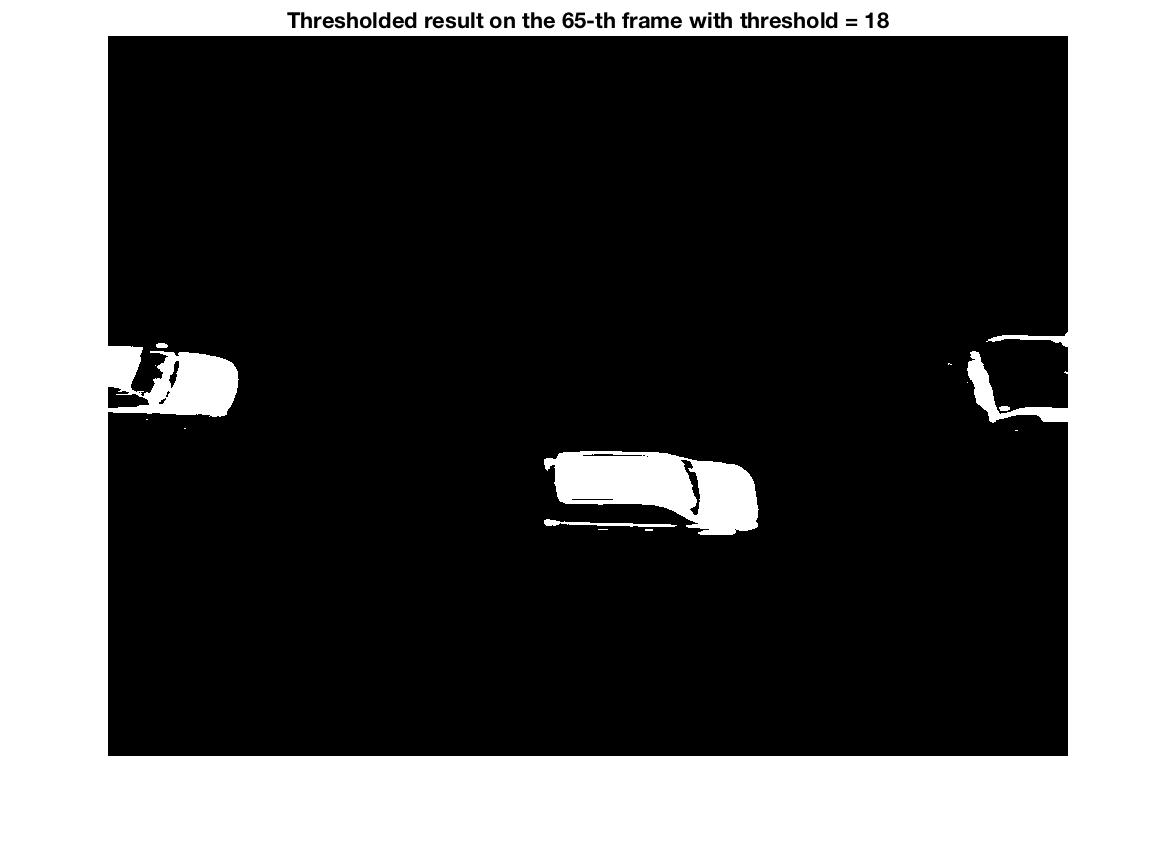
\includegraphics[width=3.4in]{2_1.jpg}
	        \caption{The thresholded result of the 65th frame}
	        \label{fig:side:a}
	    \end{minipage}%
	  \begin{minipage}[t]{0.5\textwidth}
	      \centering
	      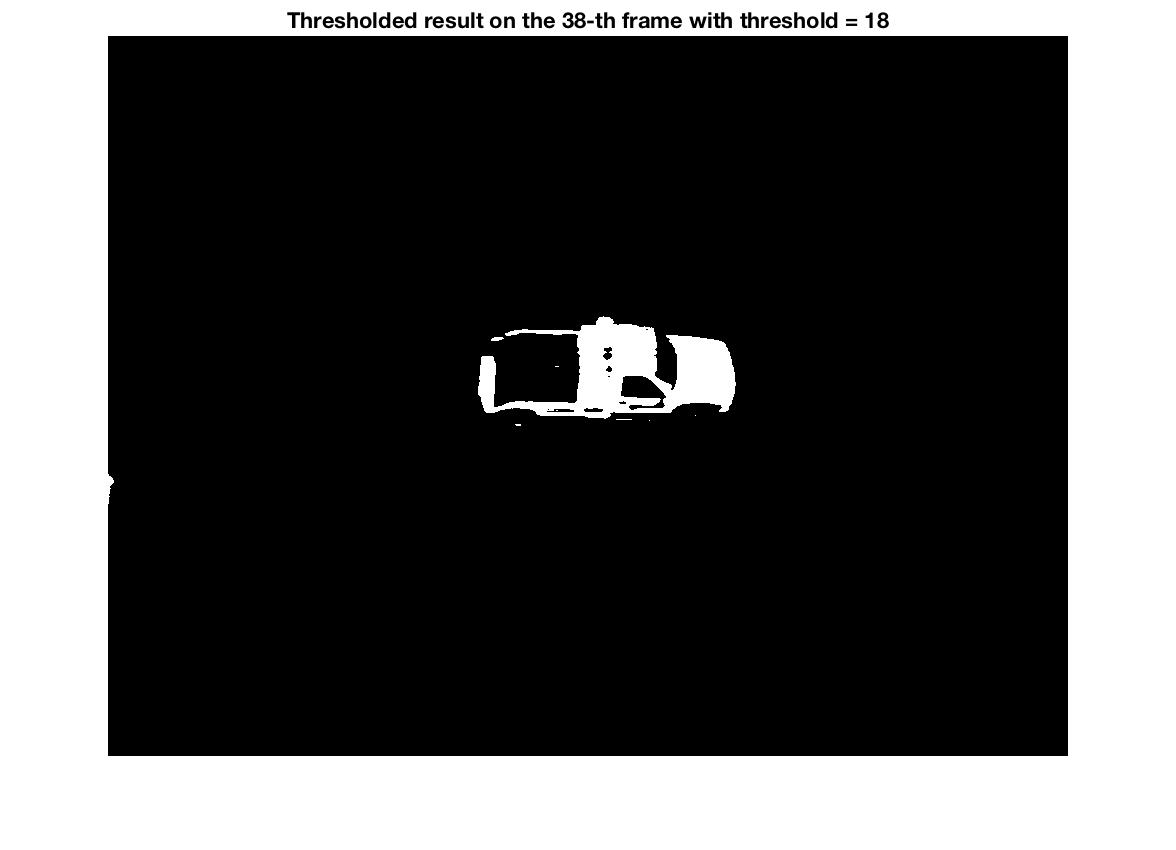
\includegraphics[width=3.4in]{2_2.jpg}
	      \caption{The thresholded result of the 38th frame}
	      \label{fig:side:b}
	    \end{minipage}
	\end{figure}
	
	\begin{figure}[H]
	    \begin{minipage}[t]{0.5\textwidth}
	        \centering
	        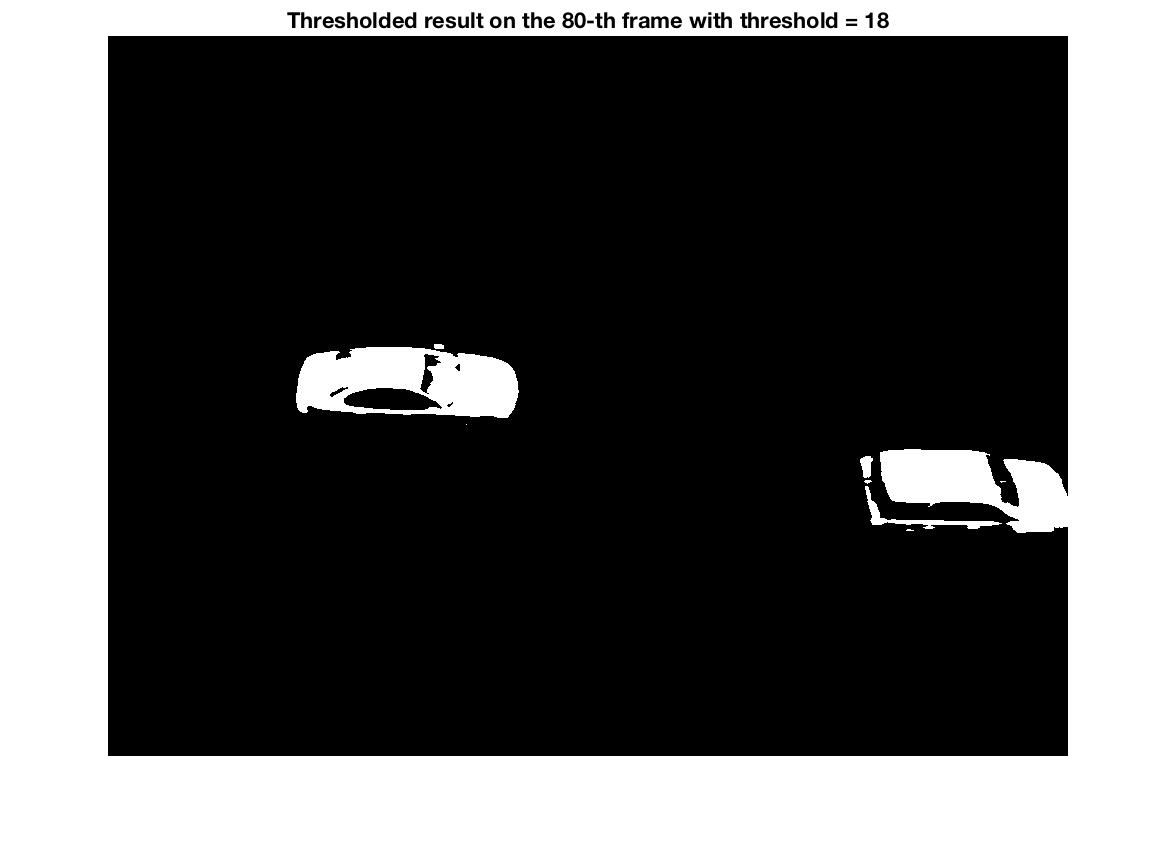
\includegraphics[width=3.4in]{2_3.jpg}
	        \caption{The thresholded result of the 80th frame}
	        \label{fig:side:a}
	    \end{minipage}%
	  \begin{minipage}[t]{0.5\textwidth}
	      \centering
	      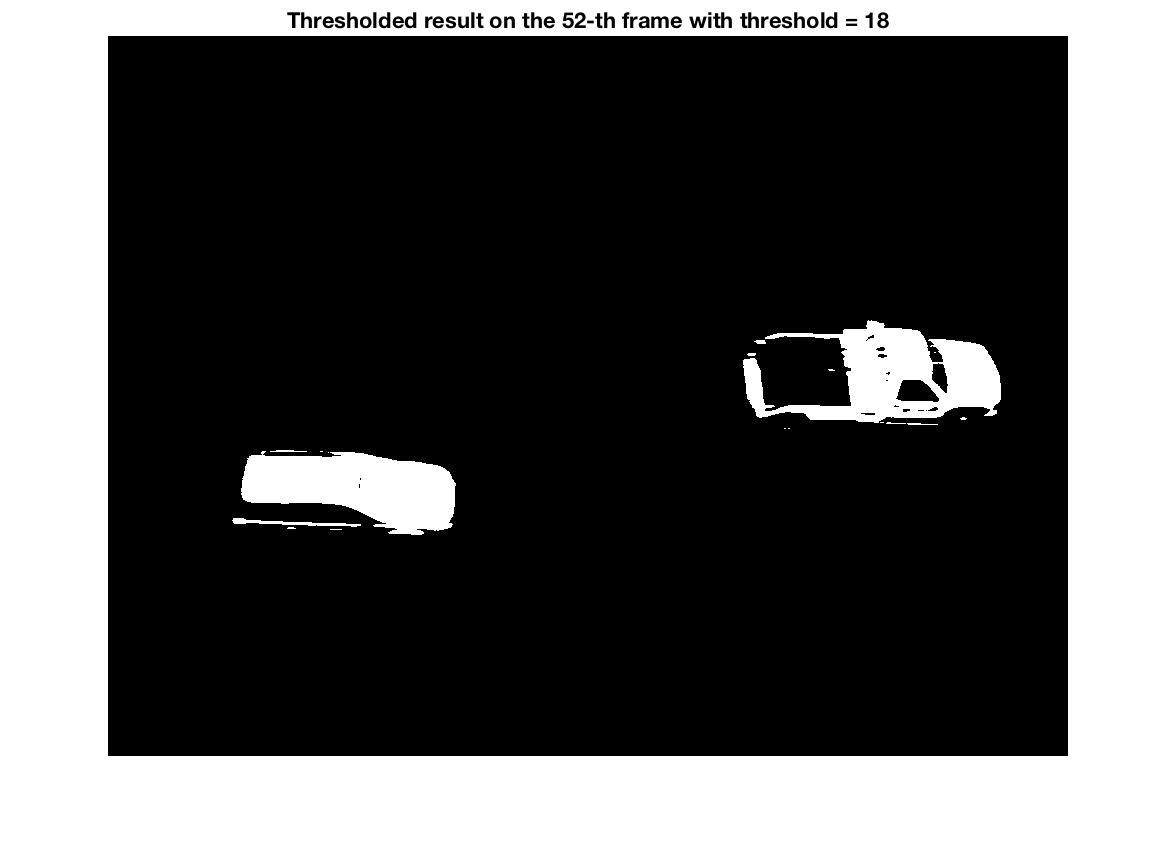
\includegraphics[width=3.4in]{2_4.jpg}
	      \caption{The thresholded result of the 52nd frame}
	      \label{fig:side:b}
	    \end{minipage}
	\end{figure}
	
	\begin{figure}[H]
	    \begin{minipage}[t]{0.5\textwidth}
	        \centering
	        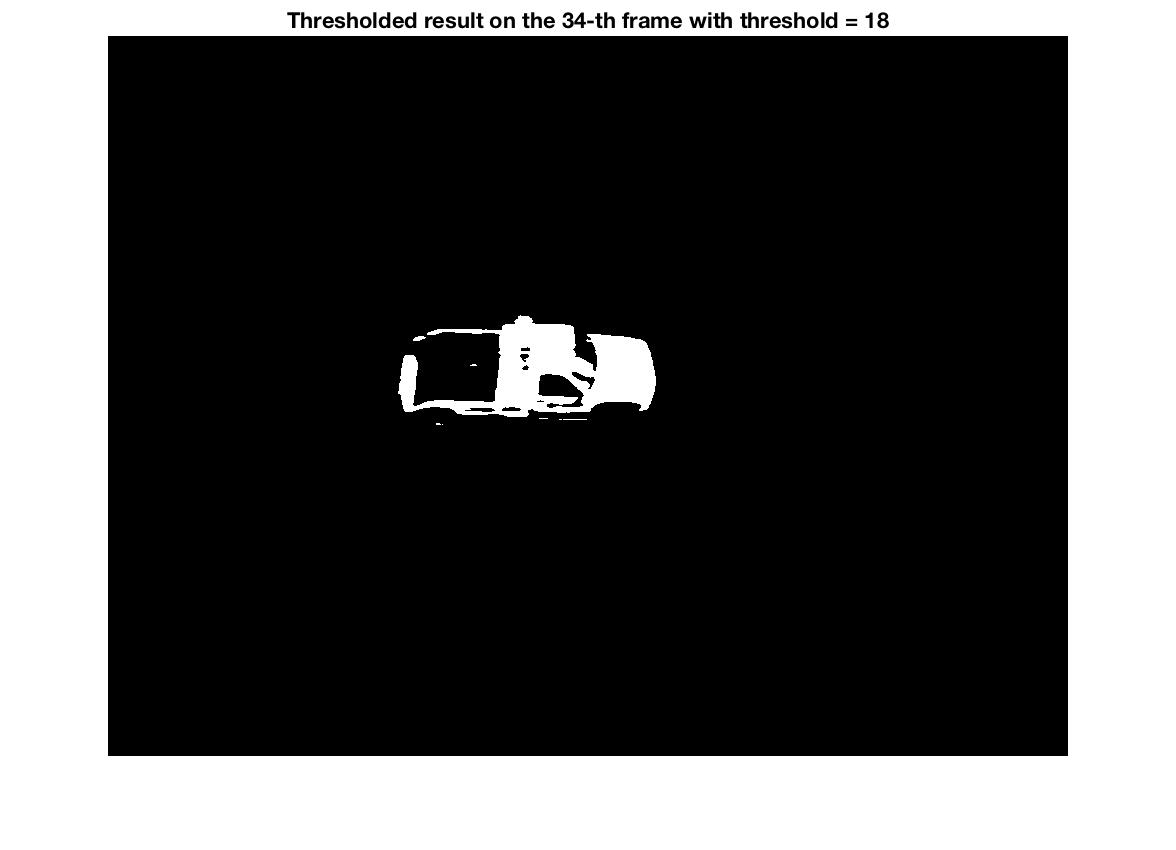
\includegraphics[width=3.4in]{2_5.jpg}
	        \caption{The thresholded result of the 34th frame}
	        \label{fig:side:a}
	    \end{minipage}%
	  \begin{minipage}[t]{0.5\textwidth}
	      \centering
	      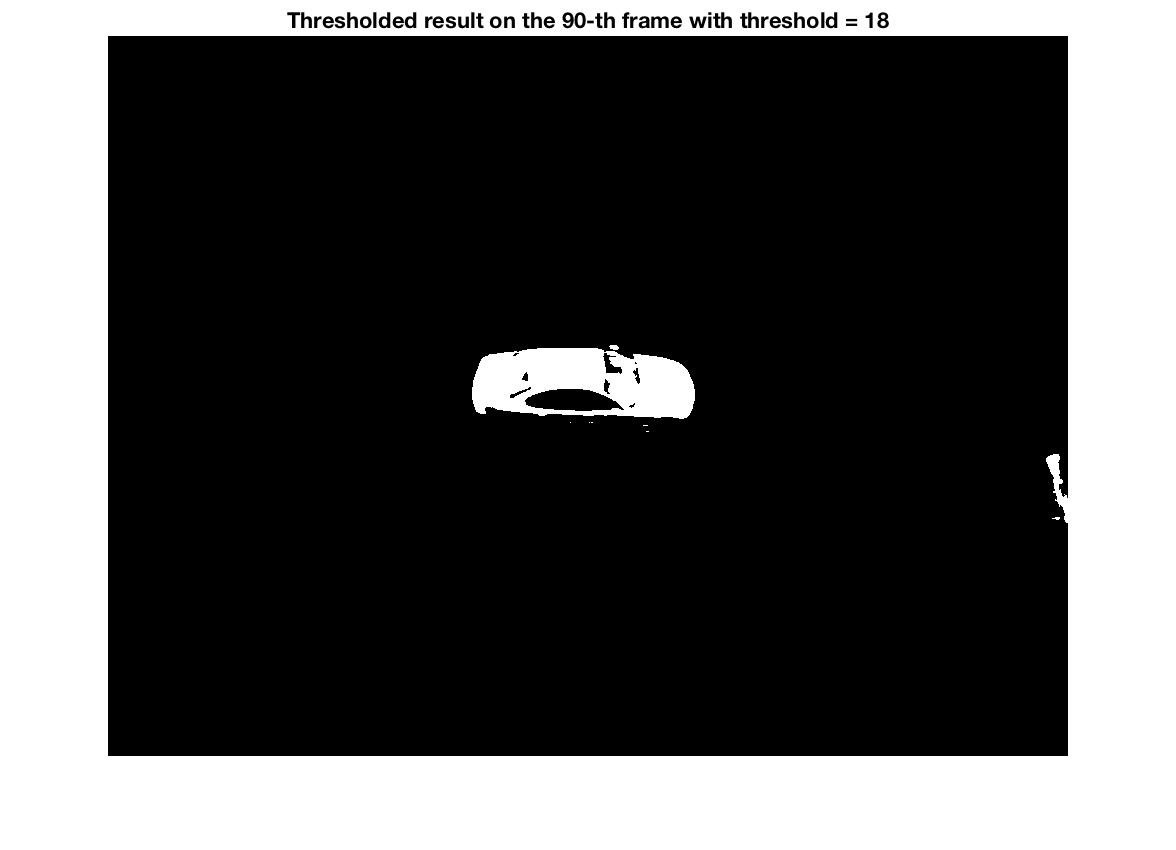
\includegraphics[width=3.4in]{2_6.jpg}
	      \caption{The thresholded result of the 90th frame}
	      \label{fig:side:b}
	    \end{minipage}
	\end{figure}
	
	\begin{figure}[H]
	    \begin{minipage}[t]{0.5\textwidth}
	        \centering
	        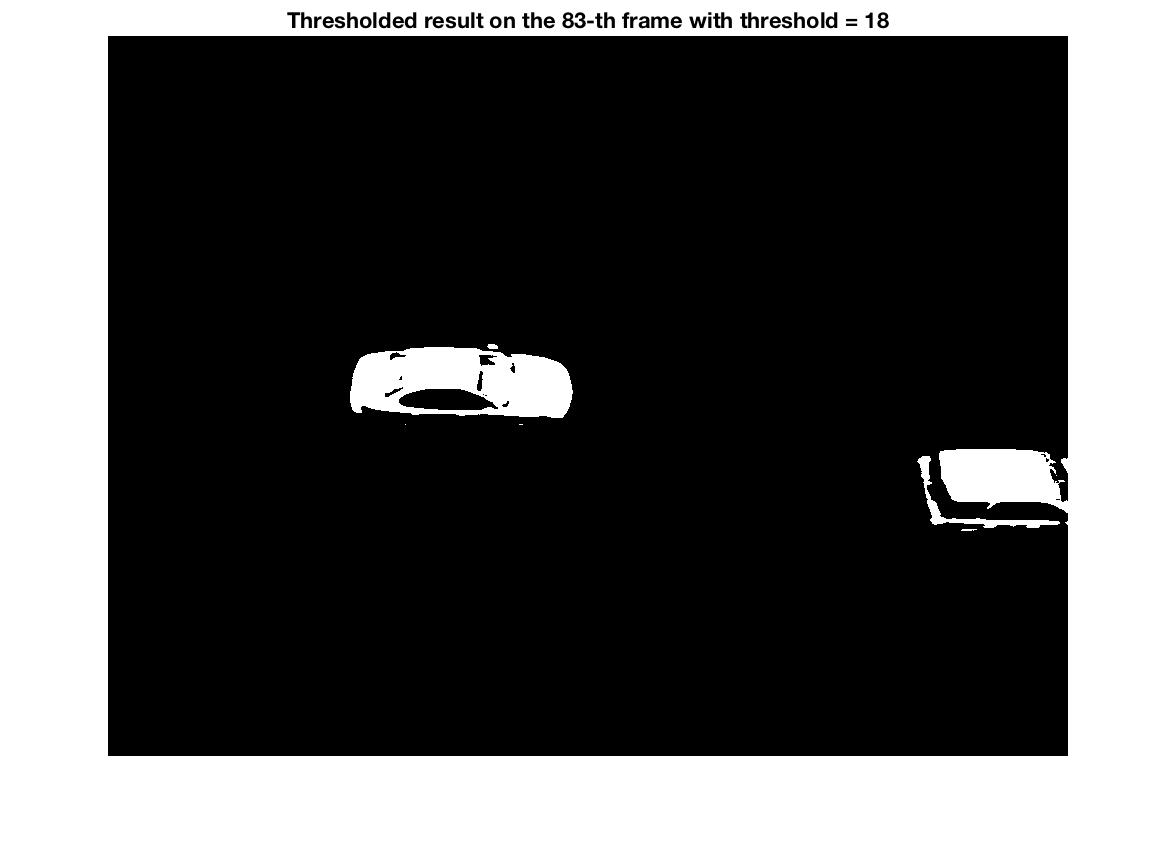
\includegraphics[width=3.4in]{2_7.jpg}
	        \caption{The thresholded result of the 83rd frame}
	        \label{fig:side:a}
	    \end{minipage}%
	  \begin{minipage}[t]{0.5\textwidth}
	      \centering
	      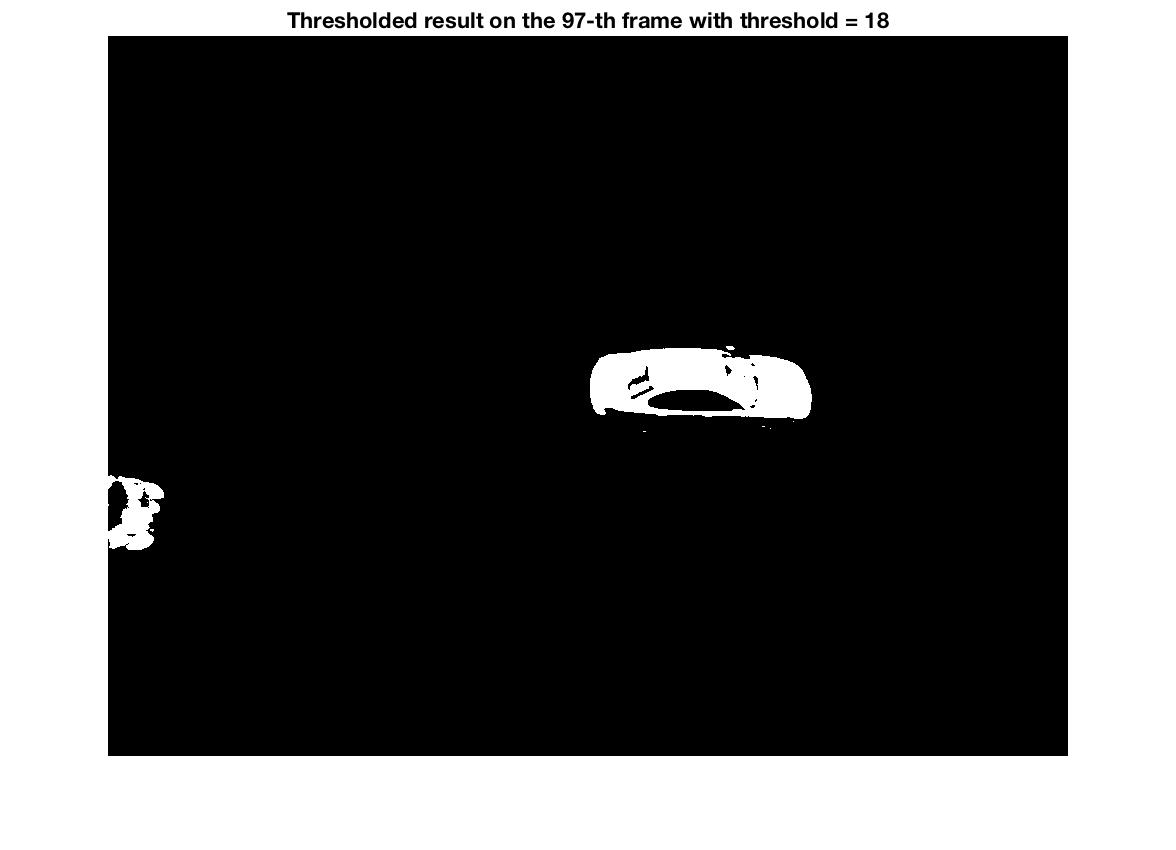
\includegraphics[width=3.4in]{2_8.jpg}
	      \caption{The thresholded result of the 97th frame}
	      \label{fig:side:b}
	    \end{minipage}
	\end{figure}
	
	\begin{figure}[H]
	    \begin{minipage}[t]{0.5\textwidth}
	        \centering
	        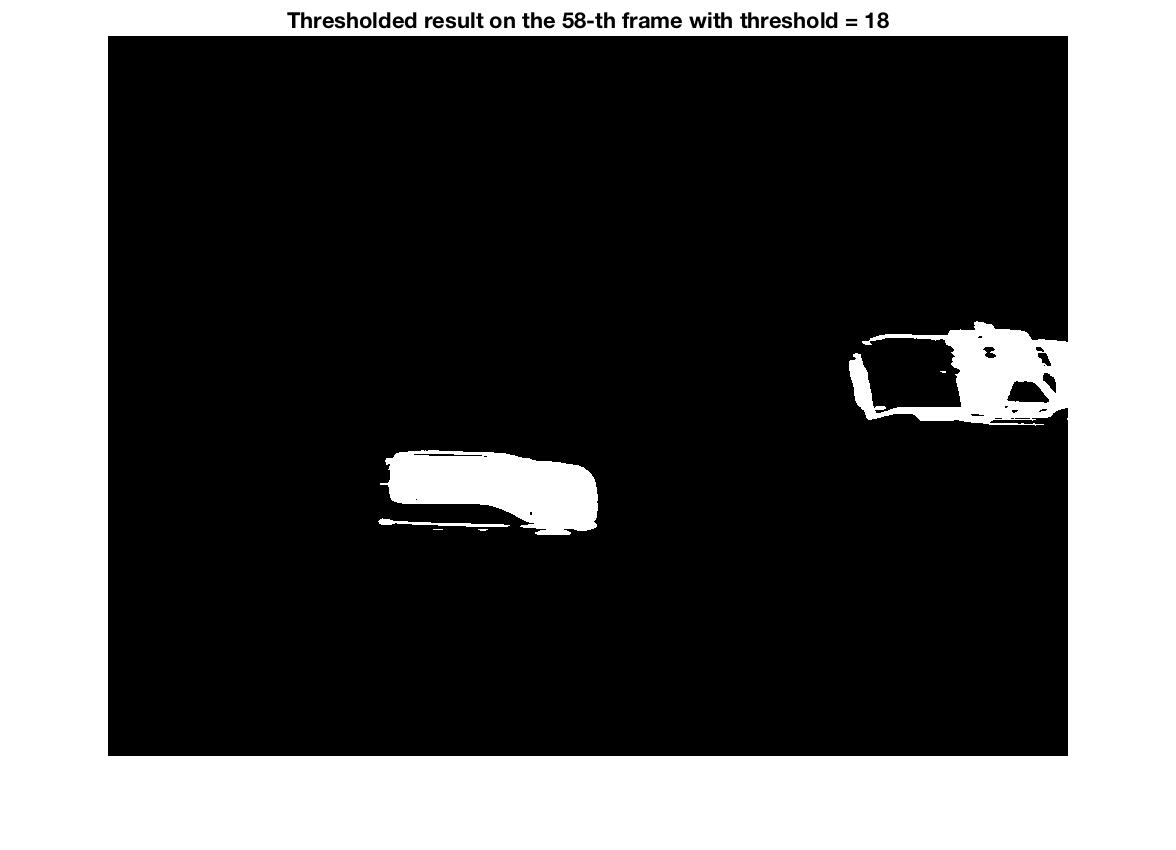
\includegraphics[width=3.4in]{2_9.jpg}
	        \caption{The thresholded result of the 58th frame}
	        \label{fig:side:a}
	    \end{minipage}%
	  \begin{minipage}[t]{0.5\textwidth}
	      \centering
	      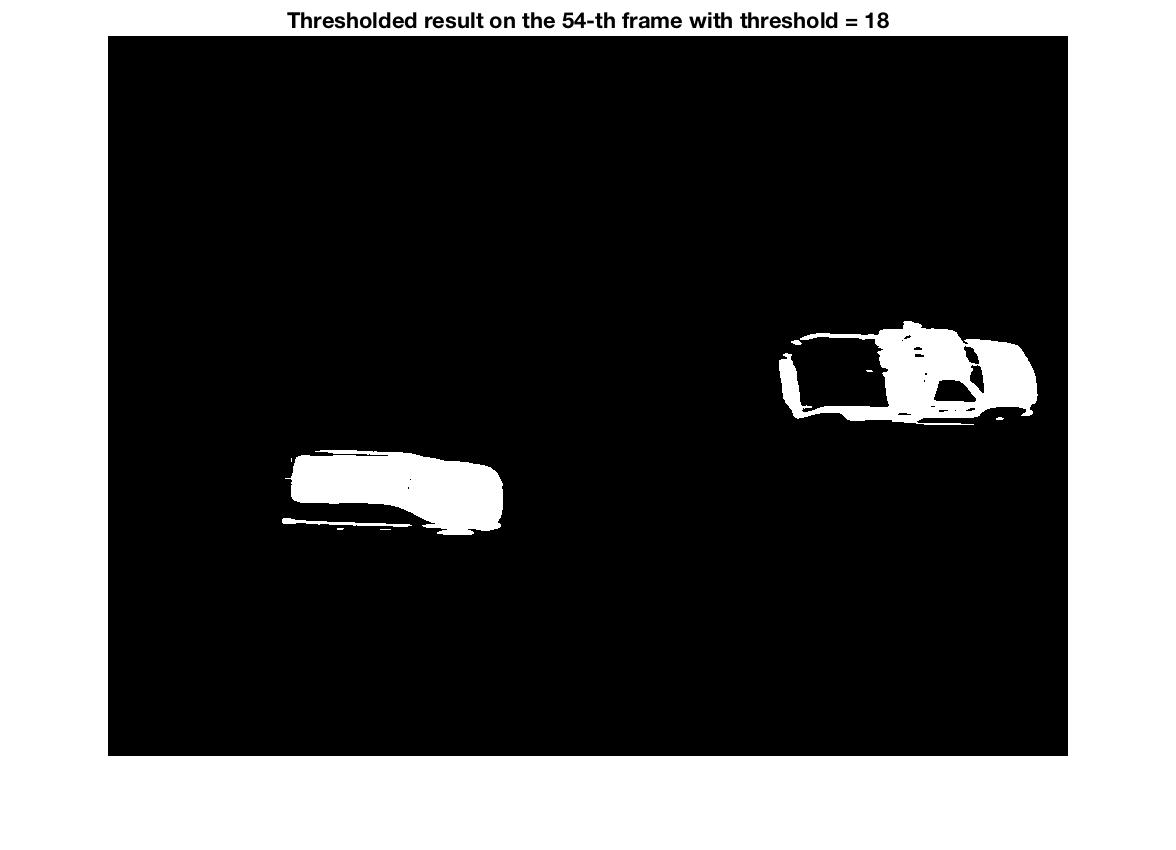
\includegraphics[width=3.4in]{2_10.jpg}
	      \caption{The thresholded result of the 54th frame}
	      \label{fig:side:b}
	    \end{minipage}
	\end{figure}
	
	\end{enumerate}
	
\end{spacing}
\end{document}